\subsection{菜单界面设计}
类别界面应考虑

导航漫游记录以 3D 界面形式呈现。如图\ref{fig:d-03}。

\begin{figure}[htp]
\centering
\fbox{
  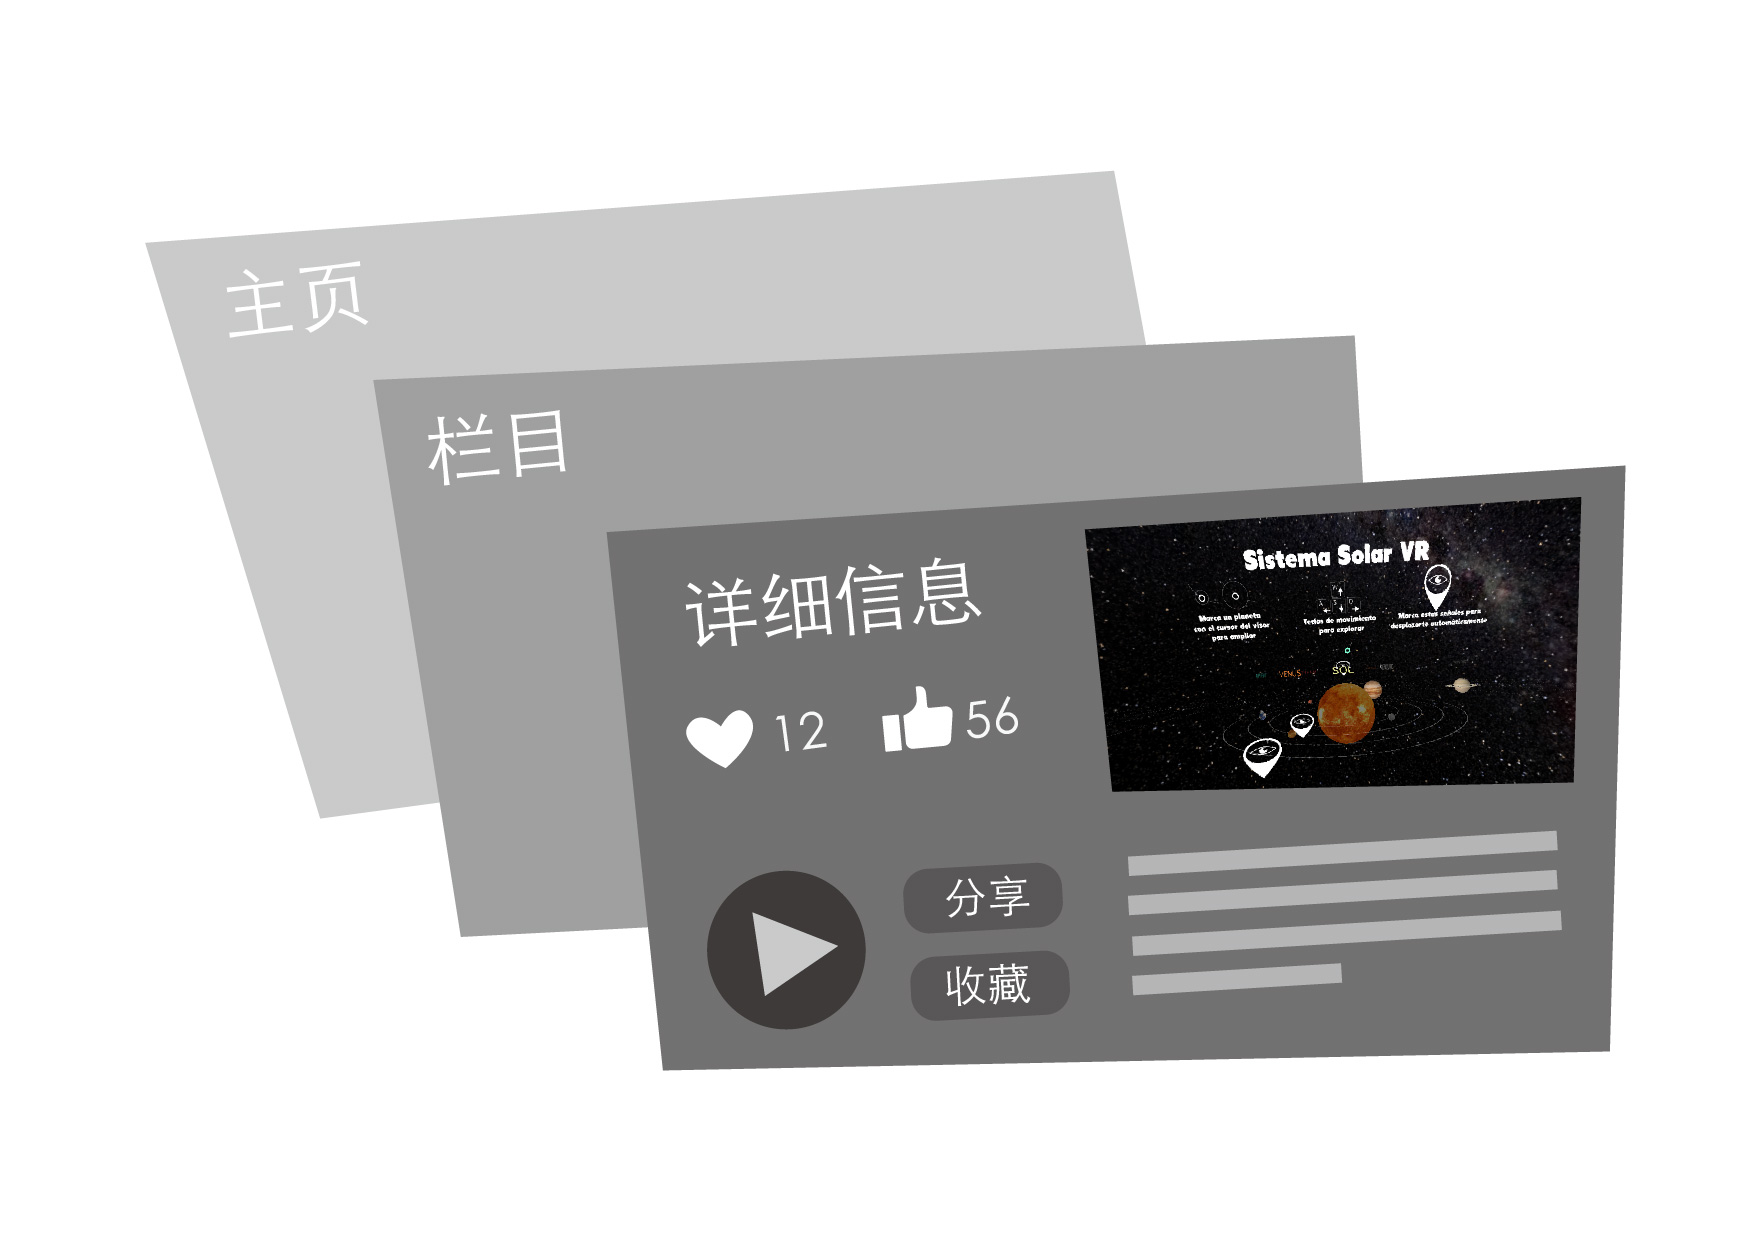
\includegraphics[width=.5\textwidth]{design/d-03}
}
\caption{3D界面}
\label{fig:d-03}
\end{figure}

主界面如图\ref{fig:d-01}。

\begin{figure}[htp]
\centering
\fbox{
  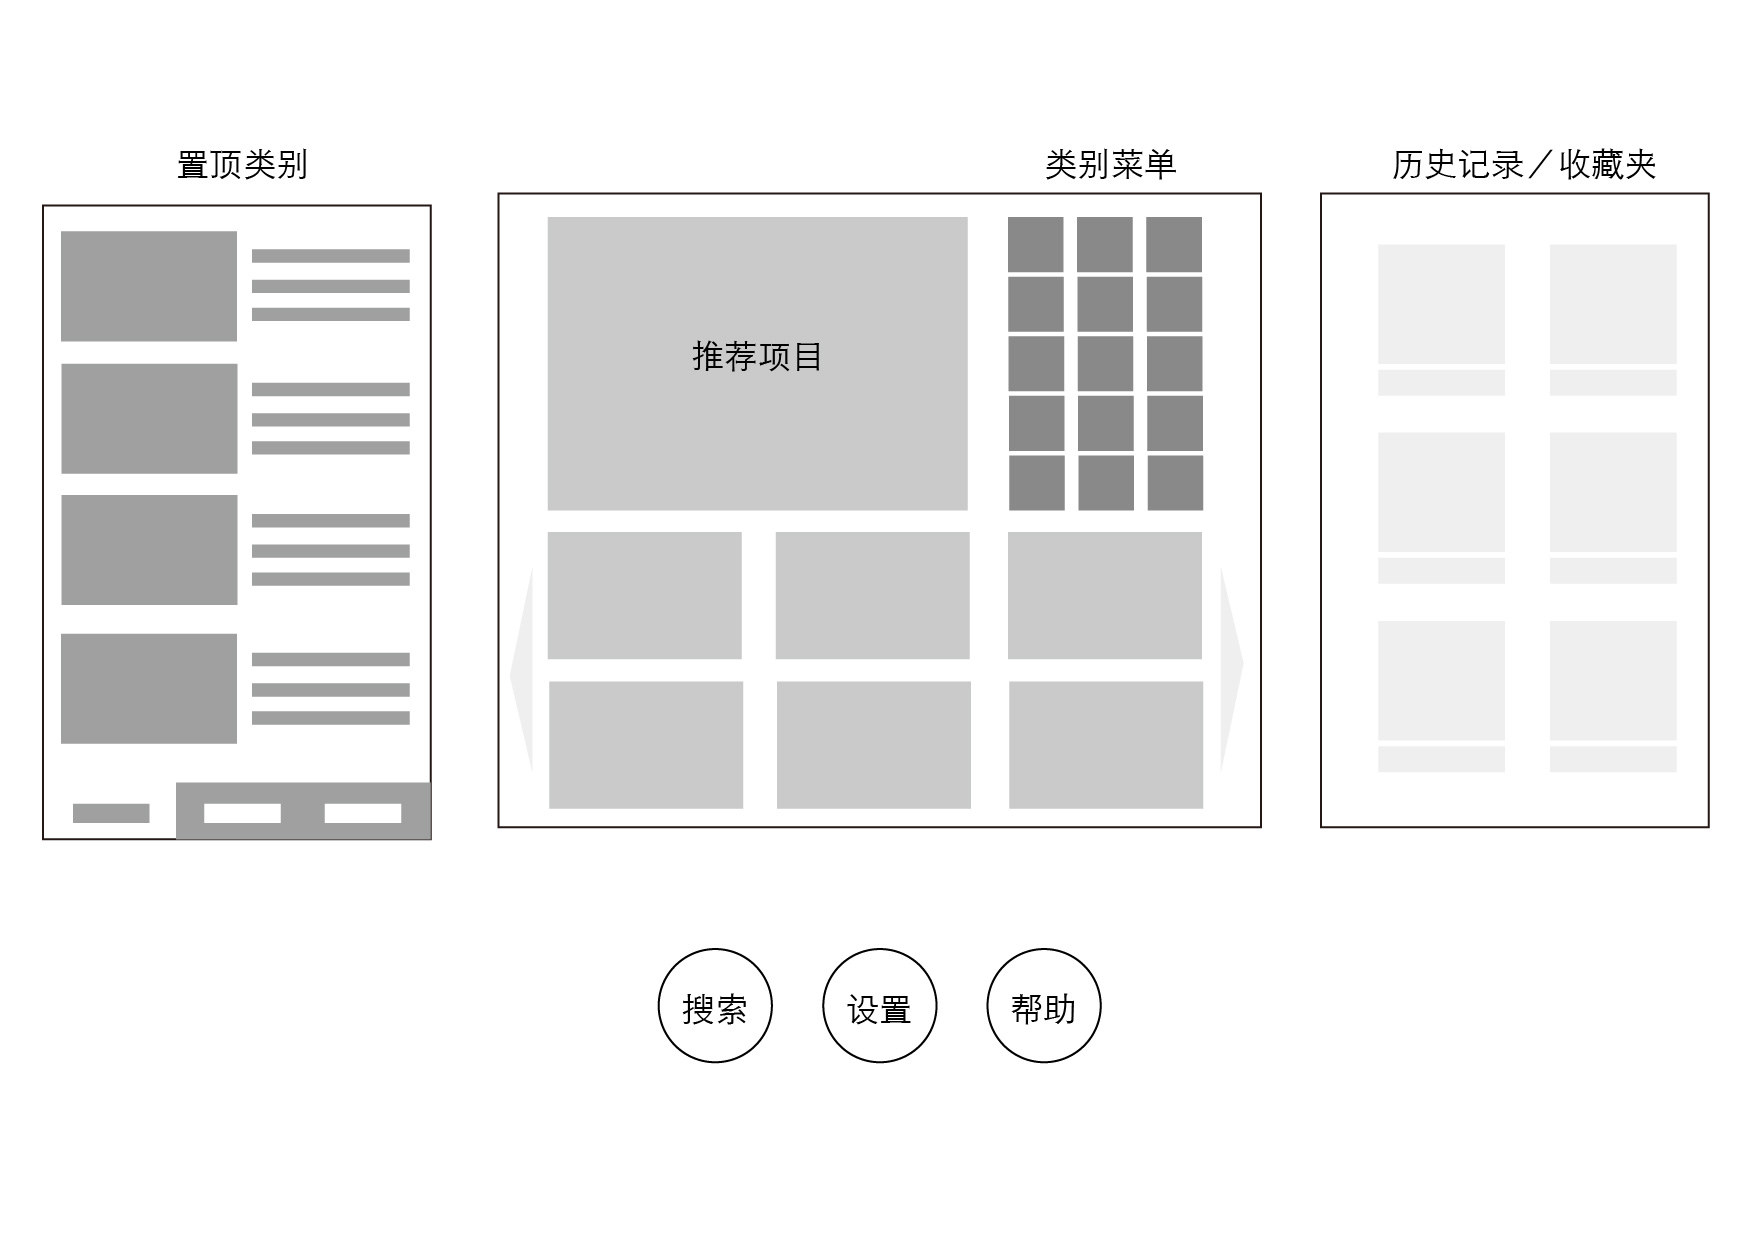
\includegraphics[width=.5\textwidth]{design/d-01}
}
\caption{主界面}
\label{fig:d-01}
\end{figure}

类别界面如图\ref{fig:d-06}。

\begin{figure}[htp]
\centering
\fbox{
  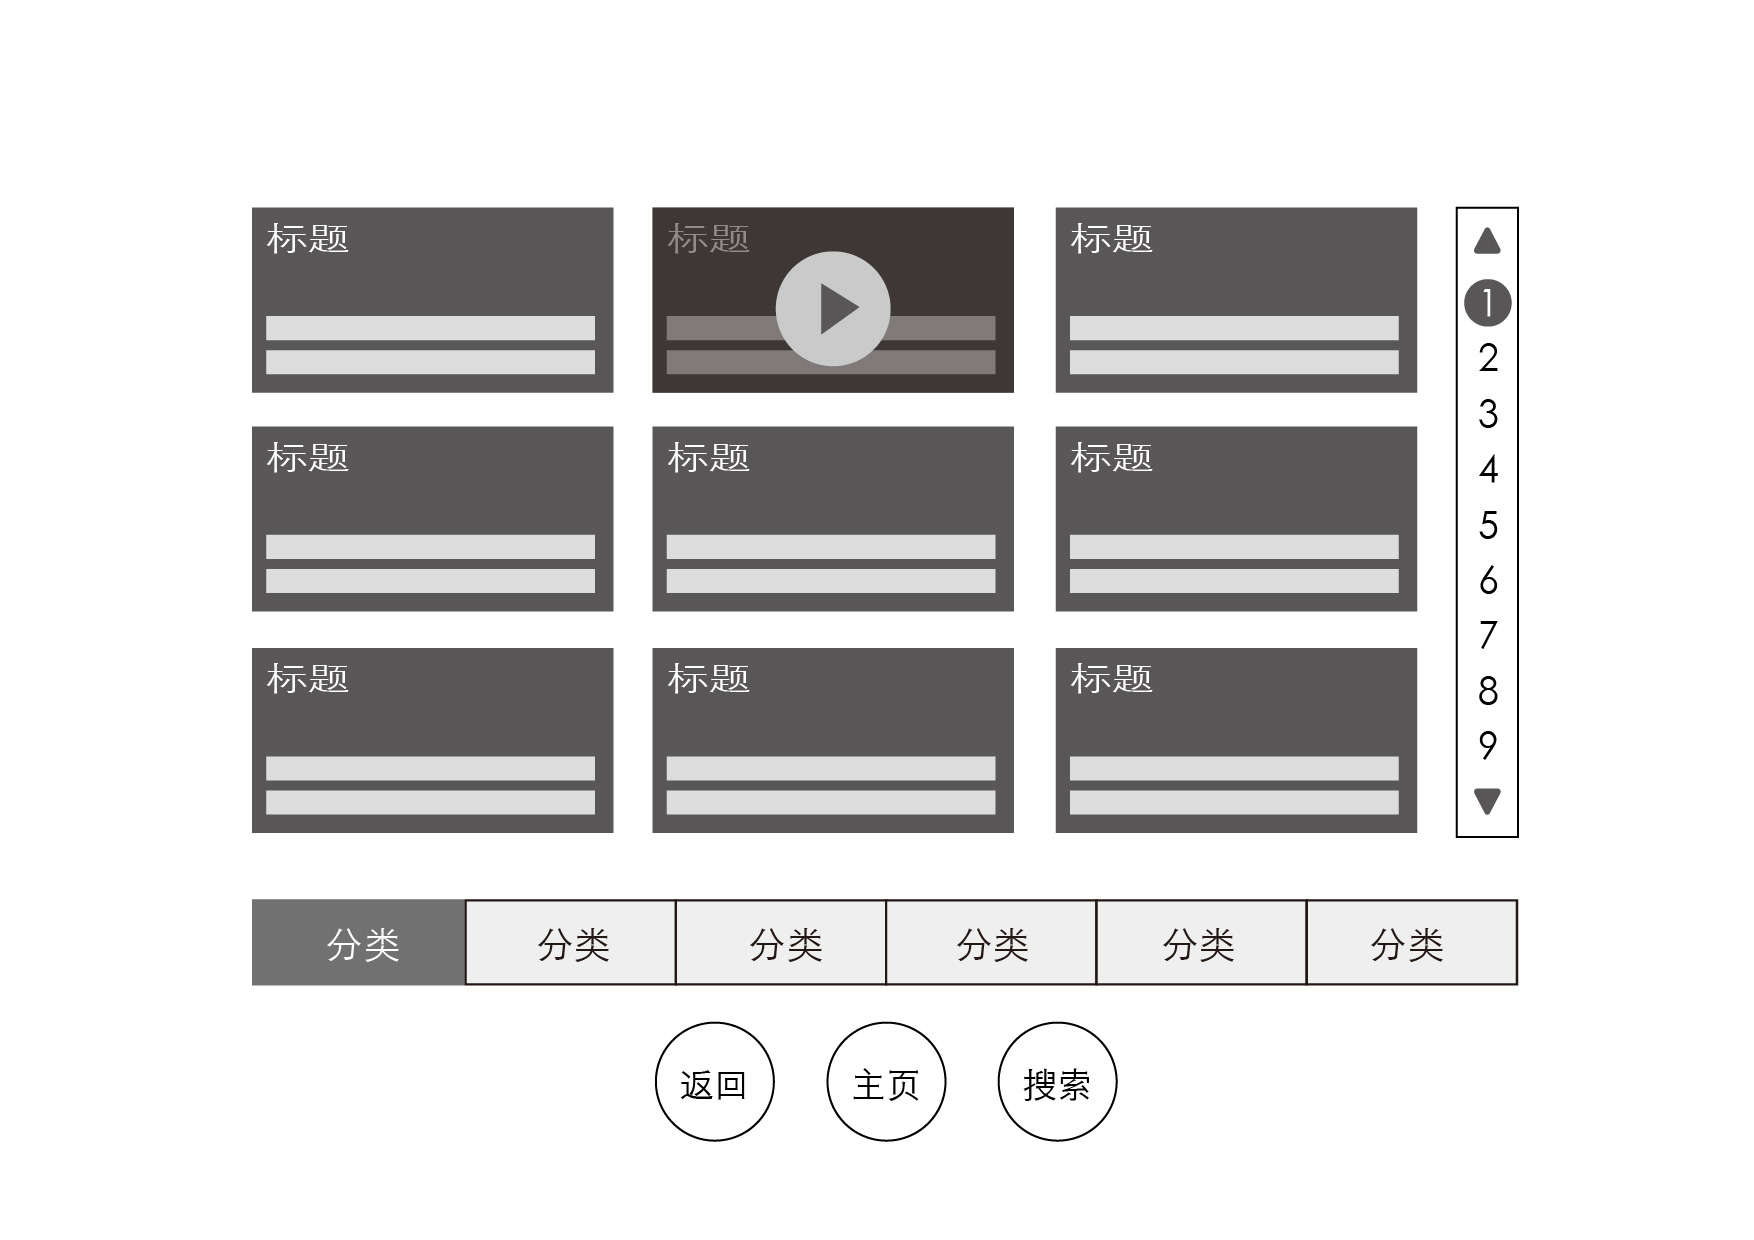
\includegraphics[width=.5\textwidth]{design/d-06}
}
\caption{类别界面}
\label{fig:d-06}
\end{figure}

考虑到存在用户偏向物理存在感强的菜单界面,故也有仿星系运动的界面如图\ref{fig:d-02}。

\begin{figure}[htp]
\centering
\fbox{
  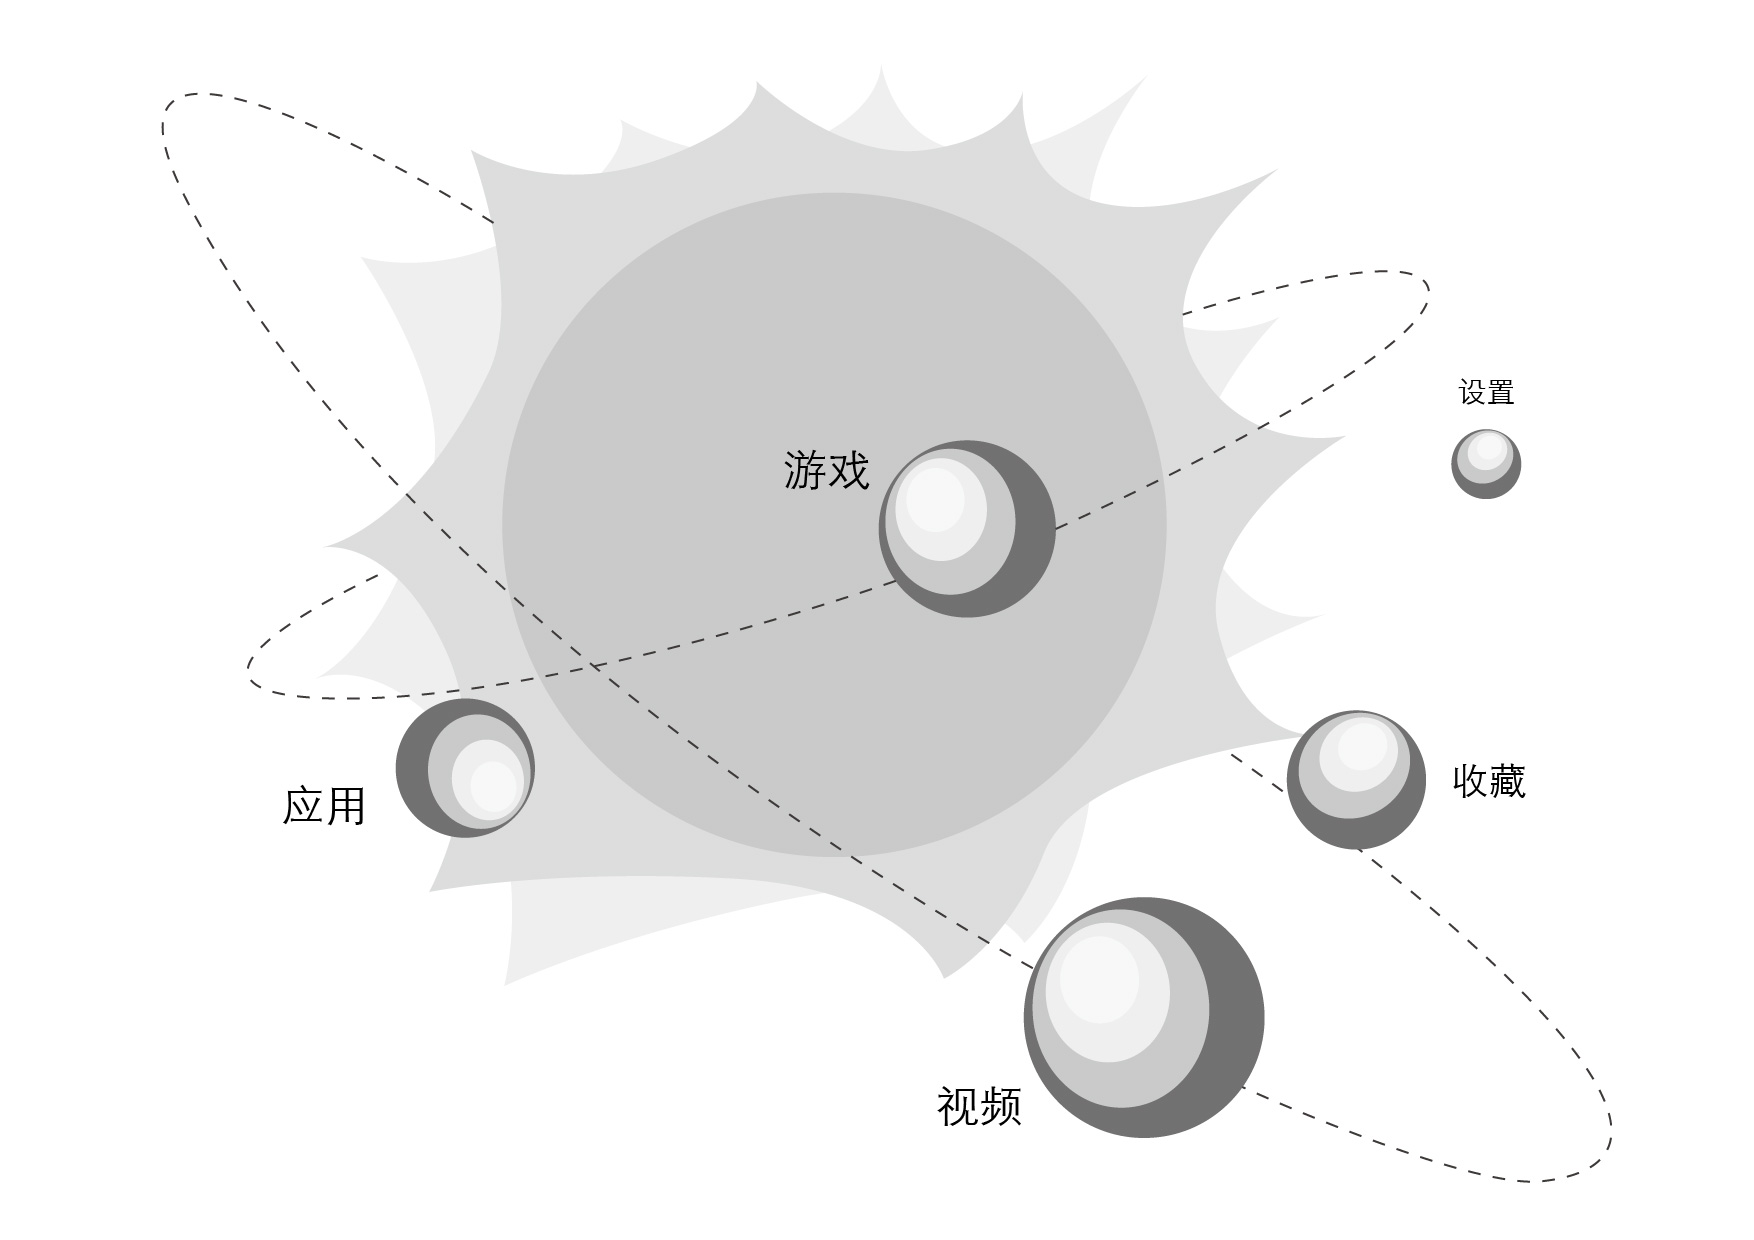
\includegraphics[width=.5\textwidth]{design/d-02}
}
\caption{星系状界面}
\label{fig:d-02}
\end{figure}

单个场景详情界面如图\ref{fig:d-07}。

\begin{figure}[htp]
\centering
\fbox{
  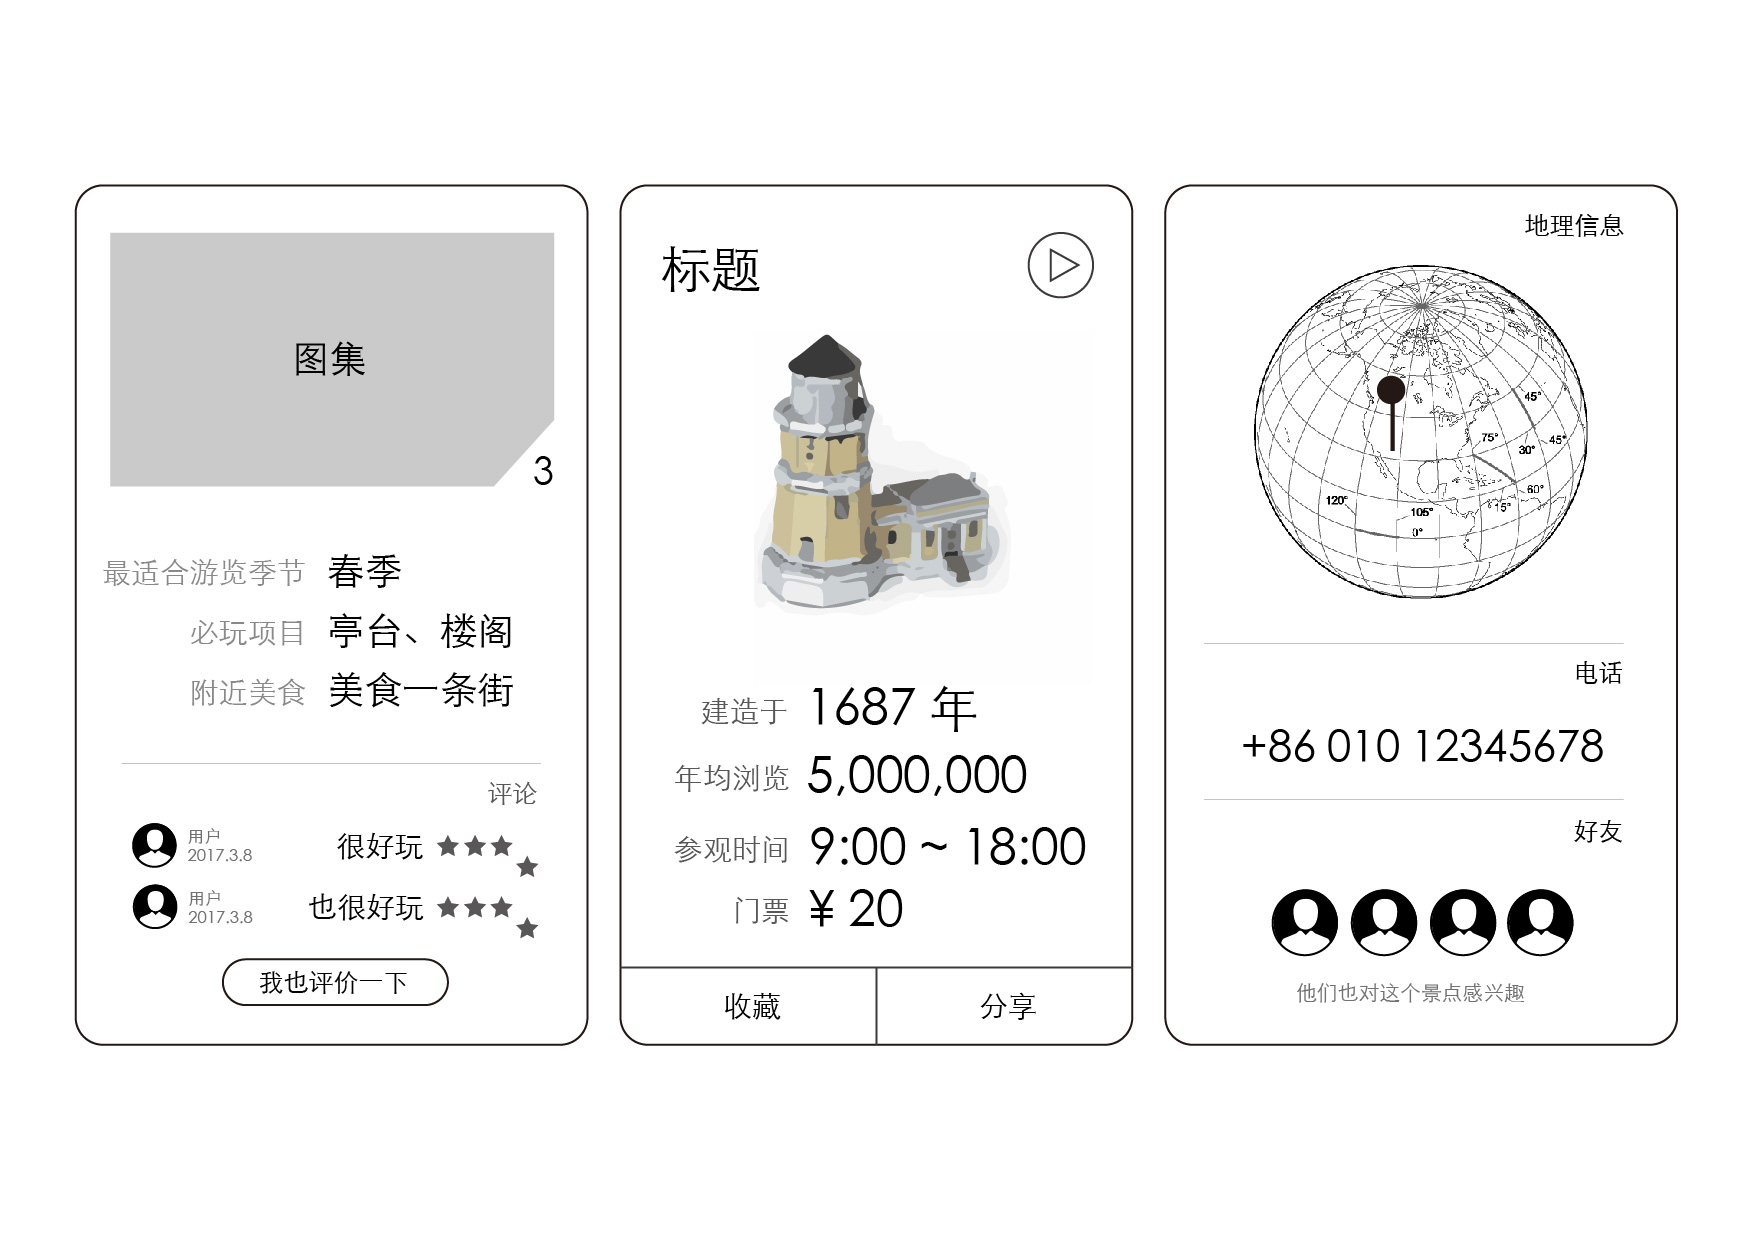
\includegraphics[width=.5\textwidth]{design/d-07}
}
\caption{单个场景详情界面}
\label{fig:d-07}
\end{figure}

\subsection{漫游界面设计}
\begin{itemize}
	\item 漫游界面带有紧急退出区域,只需注视 1~2 秒以上就可以紧急退出场景,避免眩晕加重。
	\item 可通过地面上的指示图标切换场景。
	\item 可通过场景中的热点区域查看详细信息。
\end{itemize}
如图\ref{fig:scenery}。

\begin{figure}[htp]
\centering
\fbox{
  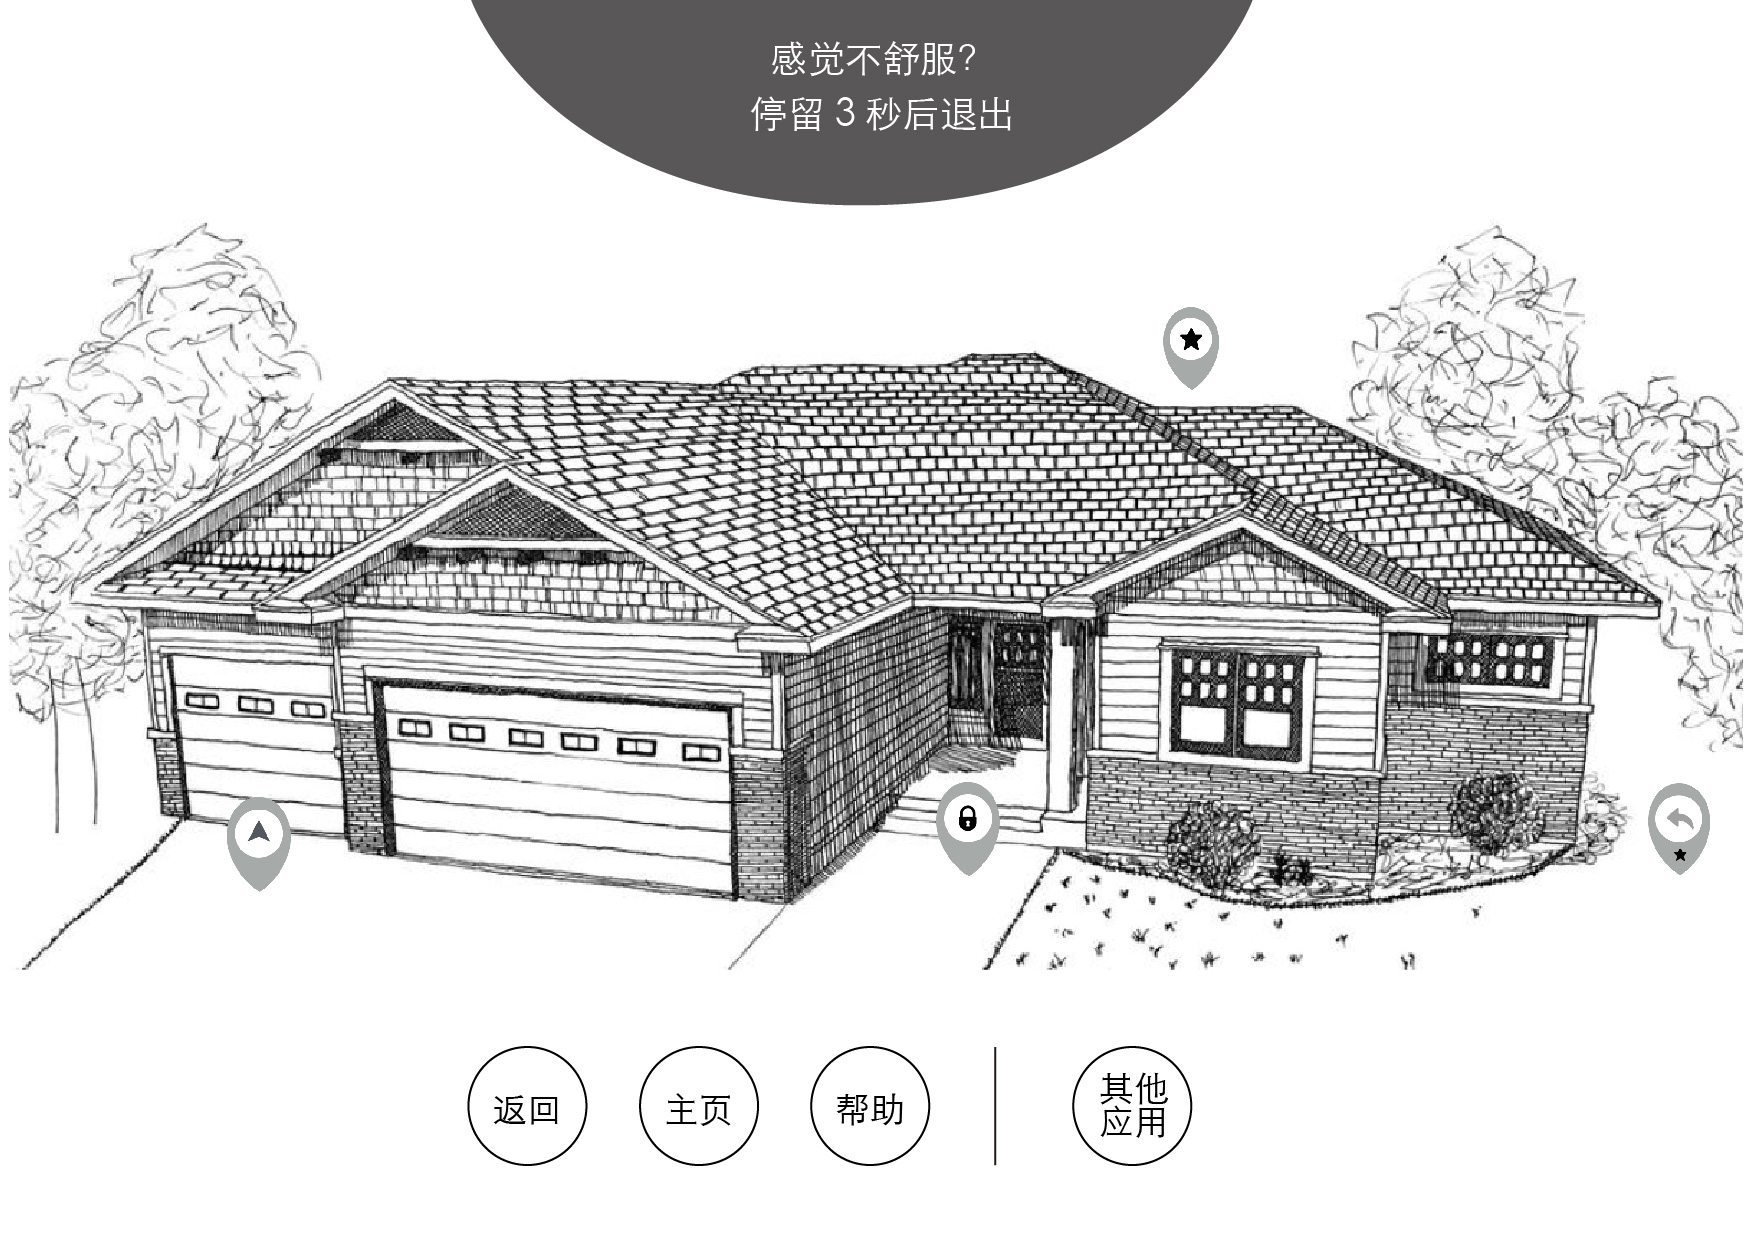
\includegraphics[width=.5\textwidth]{design/d-08}
}
\caption{漫游界面设计}
\label{fig:scenery}
\end{figure}

\subsection{功能界面设计}

语音搜索界面如图\ref{fig:d-04}。

\begin{figure}[htp]
\centering
\fbox{
  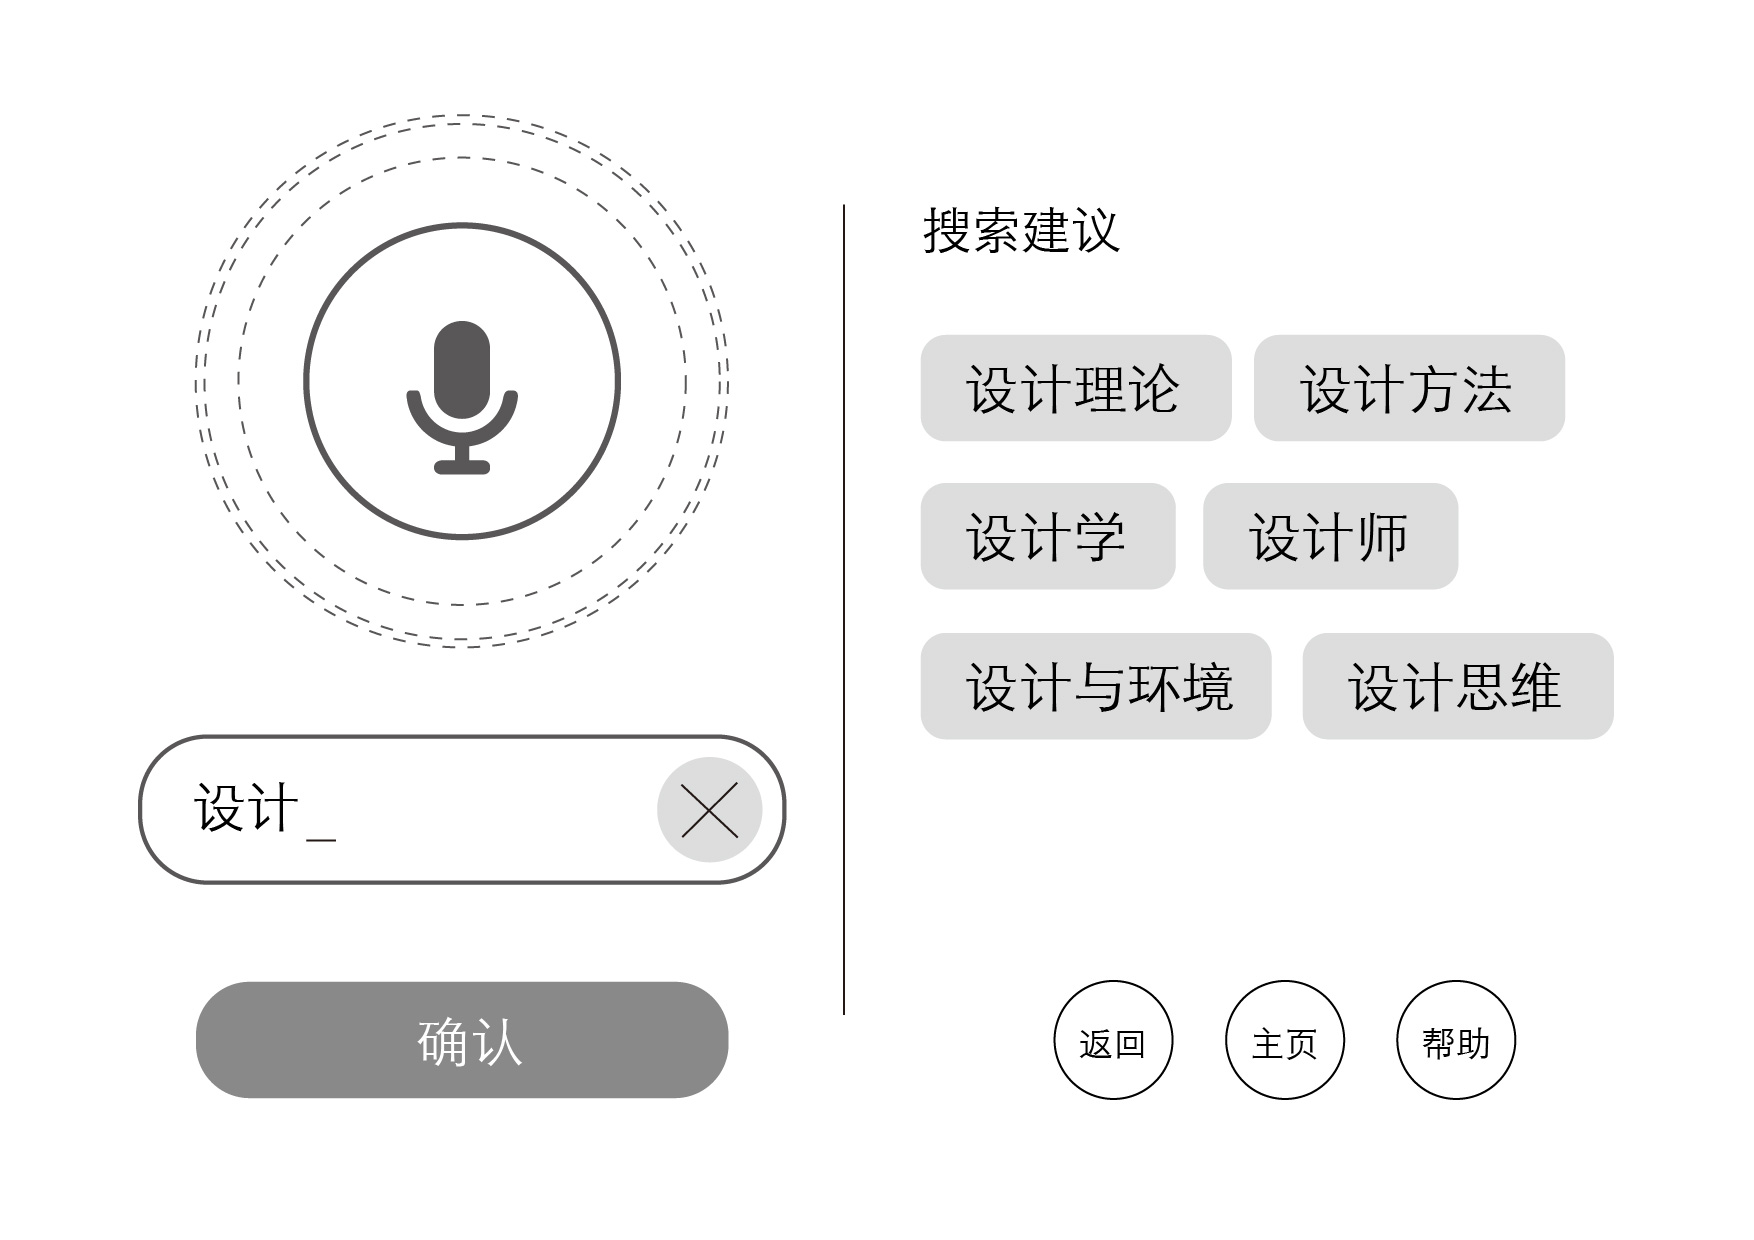
\includegraphics[width=.5\textwidth]{design/d-04}
}
\caption{语音搜索界面}
\label{fig:d-04}
\end{figure}

设置界面如图\ref{fig:d-05}。

\begin{figure}[htp]
\centering
\fbox{
  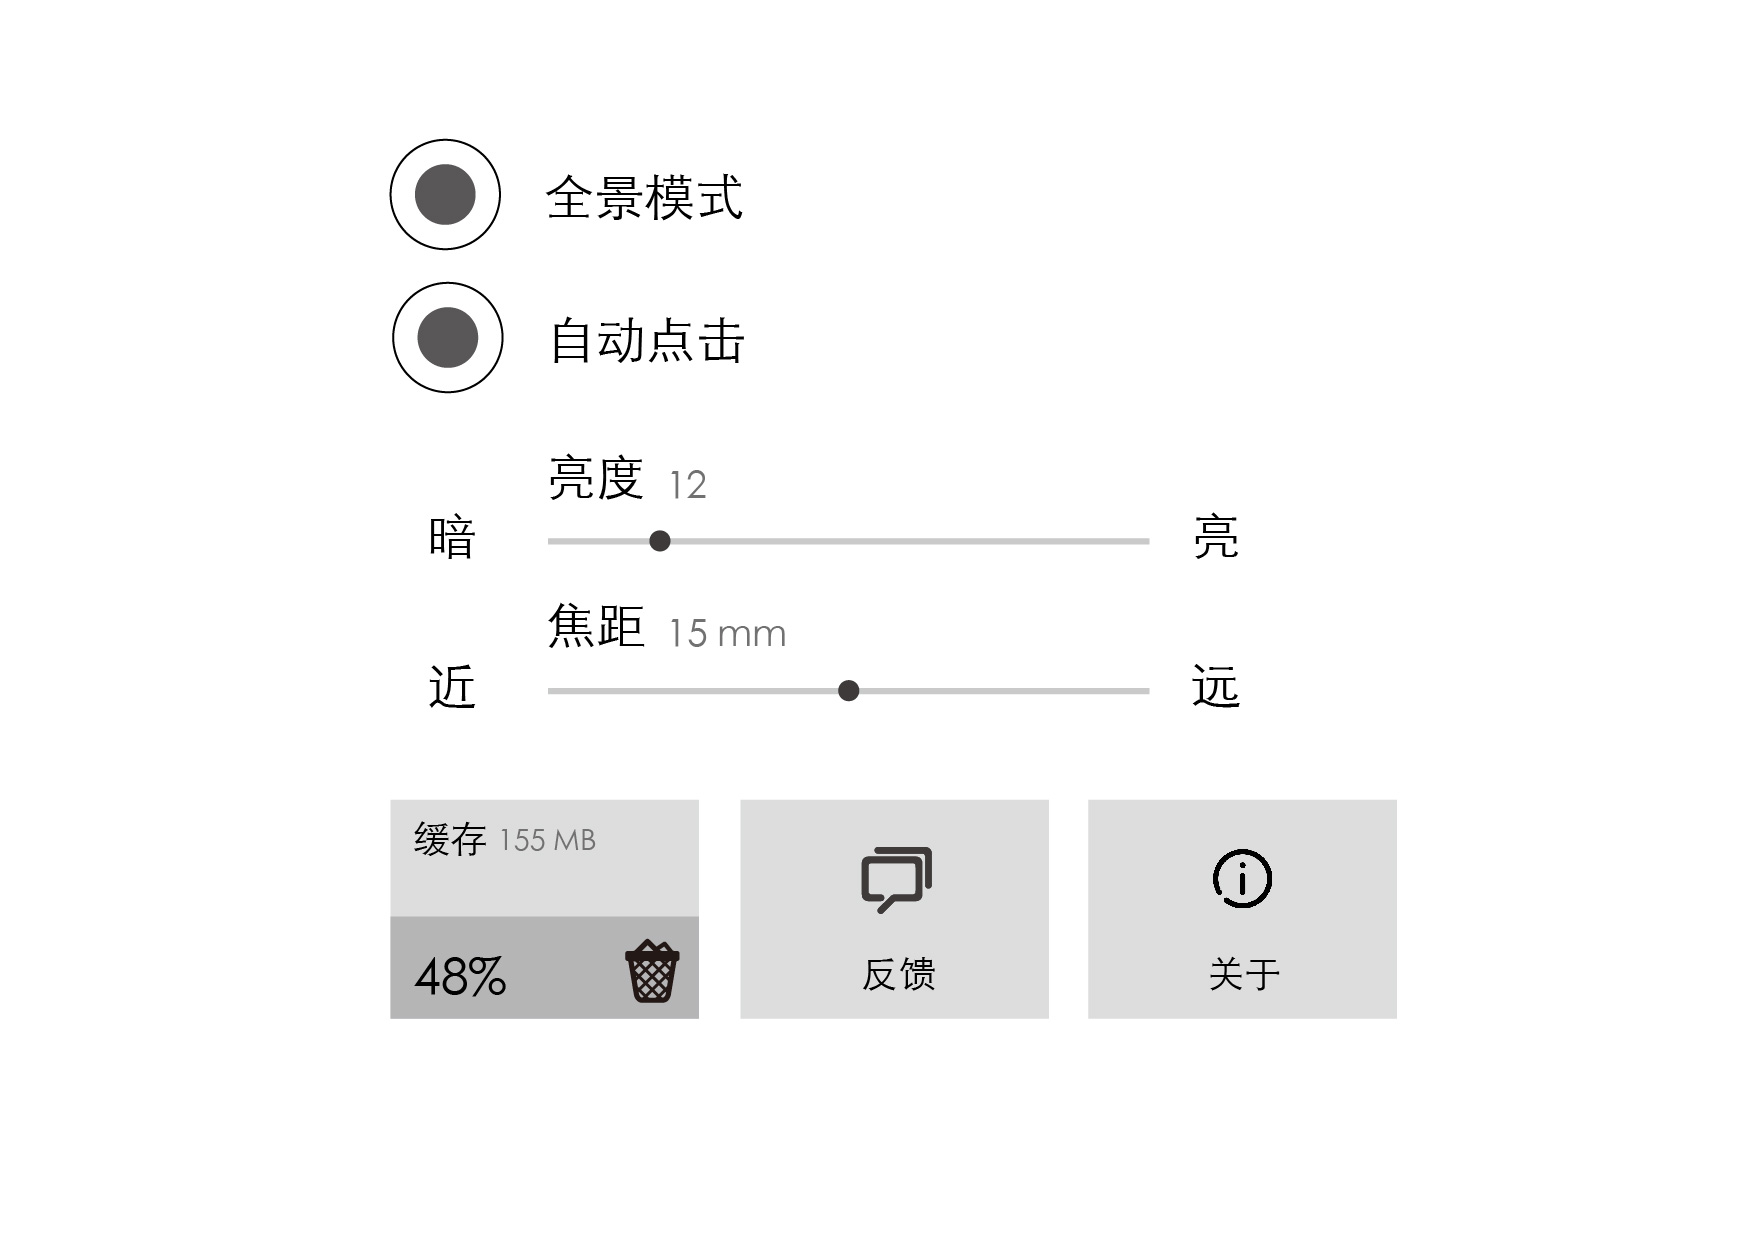
\includegraphics[width=.5\textwidth]{design/d-05}
}
\caption{设置界面}
\label{fig:d-05}
\end{figure}